\chapter*{Annexes}
\addcontentsline{toc}{chapter}{Annexes}
\markboth{Annexes}{Annexes}
\setcounter{table}{0}\setcounter{figure}{0}
\renewcommand{\thetable}{A.\arabic{table}}\renewcommand{\thefigure}{A.\arabic{figure}}
\setlength{\emergencystretch}{2em}

\Needspace{22\baselineskip}
\section*{Annexe A : Principaux points d'accès de l'API}
\addcontentsline{toc}{section}{Annexe A : Principaux points d'accès de l'API}

{\footnotesize\setstretch{1.05}\renewcommand{\arraystretch}{1.3}\arrayrulecolor{ALtexte}
\begin{longtable}{|>{\raggedright\arraybackslash}p{1.91cm}|>{\raggedright\arraybackslash}p{5.72cm}|>{\raggedright\arraybackslash}p{2.77cm}|>{\raggedright\arraybackslash}p{3.47cm}|}
\caption{Points d'accès de l'API}\\
\hline
\rowcolor{ALbleu} \sffamily\bfseries\color{white} Méthode & \sffamily\bfseries\color{white} Route & \sffamily\bfseries\color{white} Rôle & \sffamily\bfseries\color{white} Description \\ \hline
\endfirsthead
\caption[]{Points d'accès de l'API (suite)}\\
\hline
\rowcolor{ALbleu} \sffamily\bfseries\color{white} Méthode & \sffamily\bfseries\color{white} Route & \sffamily\bfseries\color{white} Rôle & \sffamily\bfseries\color{white} Description \\ \hline
\endhead
POST & \texttt{/\allowbreak{}api/\allowbreak{}auth/\allowbreak{}login/\allowbreak{}} & public & Connexion (jeton d'accès + cookie) \\ \hline
\rowcolor{ALgris} POST & \texttt{/\allowbreak{}api/\allowbreak{}auth/\allowbreak{}refresh/\allowbreak{}}, \texttt{/\allowbreak{}api/\allowbreak{}auth/\allowbreak{}logout/\allowbreak{}} & cookie & Renouvellement, déconnexion \\ \hline
GET & \texttt{/\allowbreak{}api/\allowbreak{}auth/\allowbreak{}me/\allowbreak{}} & connecté & Profil \\ \hline
\rowcolor{ALgris} CRUD & \texttt{/\allowbreak{}api/\allowbreak{}users/\allowbreak{}} & Responsable & Administration des utilisateurs \\ \hline
CRUD & \texttt{/\allowbreak{}api/\allowbreak{}device-\allowbreak{}types/\allowbreak{}}, \texttt{/\allowbreak{}brands/\allowbreak{}}, \texttt{/\allowbreak{}device-\allowbreak{}models/\allowbreak{}}, \texttt{/\allowbreak{}faults/\allowbreak{}}, \texttt{/\allowbreak{}parts/\allowbreak{}} & lecture : tous ; écriture : Responsable & Catalogues \\ \hline
\rowcolor{ALgris} GET & \texttt{/\allowbreak{}api/\allowbreak{}devices/\allowbreak{}?search=}, \texttt{/\allowbreak{}api/\allowbreak{}devices/\allowbreak{}\{id\}/\allowbreak{}life-\allowbreak{}sheet/\allowbreak{}} & connecté & Appareils et fiche de vie \\ \hline
POST / GET & \texttt{/\allowbreak{}api/\allowbreak{}returns/\allowbreak{}} & connecté & Questionnaire de retour \\ \hline
\rowcolor{ALgris} POST & \texttt{/\allowbreak{}api/\allowbreak{}dossiers/\allowbreak{}reception/\allowbreak{}} & connecté & Réception d'un appareil \\ \hline
POST & \texttt{/\allowbreak{}api/\allowbreak{}dossiers/\allowbreak{}\{id\}/\allowbreak{}disinfection/\allowbreak{}}, \texttt{/\allowbreak{}diagnosis/\allowbreak{}}, \texttt{/\allowbreak{}repair/\allowbreak{}}, \texttt{/\allowbreak{}quality-\allowbreak{}control/\allowbreak{}}, \texttt{/\allowbreak{}stock-\allowbreak{}entry/\allowbreak{}}, \texttt{/\allowbreak{}delivery/\allowbreak{}} & connecté & Étapes du workflow \\ \hline
\rowcolor{ALgris} POST & \texttt{/\allowbreak{}api/\allowbreak{}dossiers/\allowbreak{}\{id\}/\allowbreak{}transition/\allowbreak{}}, \texttt{/\allowbreak{}photos/\allowbreak{}} & connecté ; recul : Responsable & Transition contrôlée, photos \\ \hline
GET & \texttt{/\allowbreak{}api/\allowbreak{}dashboard/\allowbreak{}}, \texttt{/\allowbreak{}api/\allowbreak{}journal/\allowbreak{}}, \texttt{/\allowbreak{}api/\allowbreak{}stock-\allowbreak{}movements/\allowbreak{}} & connecté & Indicateurs, journal, mouvements \\ \hline
\rowcolor{ALgris} GET & \texttt{/\allowbreak{}api/\allowbreak{}reports/\allowbreak{}journal.\allowbreak{}csv}, \texttt{/\allowbreak{}api/\allowbreak{}reports/\allowbreak{}dossiers.\allowbreak{}csv} & connecté / Responsable & Exports CSV \\ \hline
\end{longtable}
}

\Needspace{16\baselineskip}
\section*{Annexe B : Entités du modèle de données}
\addcontentsline{toc}{section}{Annexe B : Entités du modèle de données}

{\small\setstretch{1.05}\renewcommand{\arraystretch}{1.3}\arrayrulecolor{ALtexte}
\begin{longtable}{|>{\raggedright\arraybackslash}p{3.65cm}|>{\raggedright\arraybackslash}p{10.96cm}|}
\caption{Entités du modèle de données}\\
\hline
\rowcolor{ALbleu} \sffamily\bfseries\color{white} Groupe & \sffamily\bfseries\color{white} Entités \\ \hline
\endfirsthead
\caption[]{Entités du modèle de données (suite)}\\
\hline
\rowcolor{ALbleu} \sffamily\bfseries\color{white} Groupe & \sffamily\bfseries\color{white} Entités \\ \hline
\endhead
Utilisateurs & User (rôles : technicien, responsable SAV) \\ \hline
\rowcolor{ALgris} Référentiel d'appareils & DeviceType, Brand, DeviceModel, Device \\ \hline
Retour et dossier & ReturnDeclaration, DossierSAV, StatusHistory \\ \hline
\rowcolor{ALgris} Étapes du dossier & Disinfection, Diagnosis, DetectedFault, Repair, ReplacedPart, QualityControl, StockMovement, Delivery, Photo \\ \hline
Catalogues & Fault (pannes par type d'appareil), Part (pièces) \\ \hline
\rowcolor{ALgris} Énumérations & VisualCondition, BiohazardStatus \\ \hline
\end{longtable}
}

\Needspace{15\baselineskip}
\section*{Annexe C : Organisation du dépôt}
\addcontentsline{toc}{section}{Annexe C : Organisation du dépôt}

{\small\setstretch{1.05}\renewcommand{\arraystretch}{1.3}\arrayrulecolor{ALtexte}
\begin{longtable}{|>{\raggedright\arraybackslash}p{3.65cm}|>{\raggedright\arraybackslash}p{10.96cm}|}
\caption{Organisation du dépôt}\\
\hline
\rowcolor{ALbleu} \sffamily\bfseries\color{white} Dossier & \sffamily\bfseries\color{white} Contenu \\ \hline
\endfirsthead
\caption[]{Organisation du dépôt (suite)}\\
\hline
\rowcolor{ALbleu} \sffamily\bfseries\color{white} Dossier & \sffamily\bfseries\color{white} Contenu \\ \hline
\endhead
\texttt{backend/\allowbreak{}} & Applications Django : accounts, inventory, maintenance, dashboard, reports, common ; configuration \\ \hline
\rowcolor{ALgris} \texttt{frontend/\allowbreak{}} & Application Next.js : pages, composants, bibliothèque d'appels à l'API \\ \hline
\texttt{docs/\allowbreak{}} & Vision, cahier des charges, workflow, cas d'utilisation, architecture, base de données, API, démarrage, captures \\ \hline
\rowcolor{ALgris} \texttt{docs/\allowbreak{}diagrams/\allowbreak{}} & Sources des diagrammes UML (PlantUML, Mermaid) \\ \hline
\texttt{docker-\allowbreak{}compose.\allowbreak{}yml} & Base de données PostgreSQL 16 \\ \hline
\end{longtable}
}

\Needspace{22\baselineskip}
\section*{Annexe D : Correspondance entre le journal papier et l'application}
\addcontentsline{toc}{section}{Annexe D : Correspondance entre le journal papier et l'application}

{\small\setstretch{1.05}\renewcommand{\arraystretch}{1.3}\arrayrulecolor{ALtexte}
\begin{longtable}{|>{\raggedright\arraybackslash}p{5.02cm}|>{\raggedright\arraybackslash}p{9.59cm}|}
\caption{Correspondance journal papier / application}\\
\hline
\rowcolor{ALbleu} \sffamily\bfseries\color{white} Colonne du journal papier & \sffamily\bfseries\color{white} Origine dans AirLiquide GMAO+ \\ \hline
\endfirsthead
\caption[]{Correspondance journal papier / application (suite)}\\
\hline
\rowcolor{ALbleu} \sffamily\bfseries\color{white} Colonne du journal papier & \sffamily\bfseries\color{white} Origine dans AirLiquide GMAO+ \\ \hline
\endhead
Année, Mois & Date de réception du dossier \\ \hline
\rowcolor{ALgris} Équip. / type & Type d'appareil et modèle \\ \hline
N° série & Appareil (numéro normalisé) \\ \hline
\rowcolor{ALgris} C.H & Compteur horaire saisi à la réception \\ \hline
Pureté & Contrôle qualité (pureté O\textsubscript{2}, de 0 à 100 \%) \\ \hline
\rowcolor{ALgris} Débit / pression & Contrôle qualité \\ \hline
Alarme sonore & Contrôle qualité (conforme, non conforme, non testée) \\ \hline
\rowcolor{ALgris} Pannes & Diagnostic (pannes du catalogue) \\ \hline
Doc de sortie PR & Réparation (référence du document de sortie des pièces) \\ \hline
\rowcolor{ALgris} Technicien & Technicien de la réparation, à défaut de la désinfection \\ \hline
Date sortie & Date de livraison \\ \hline
\end{longtable}
}

Hypothèses à valider avec le service : \og{}C.H\fg{} désigne le compteur horaire ; \og{}Doc de sortie PR\fg{} désigne le document de sortie de pièces de rechange ; le dernier contrôle qualité fait foi pour les mesures.

\section*{Annexe E : Captures complémentaires}
\addcontentsline{toc}{section}{Annexe E : Captures complémentaires}

\begin{figure}[!htb]
\centering
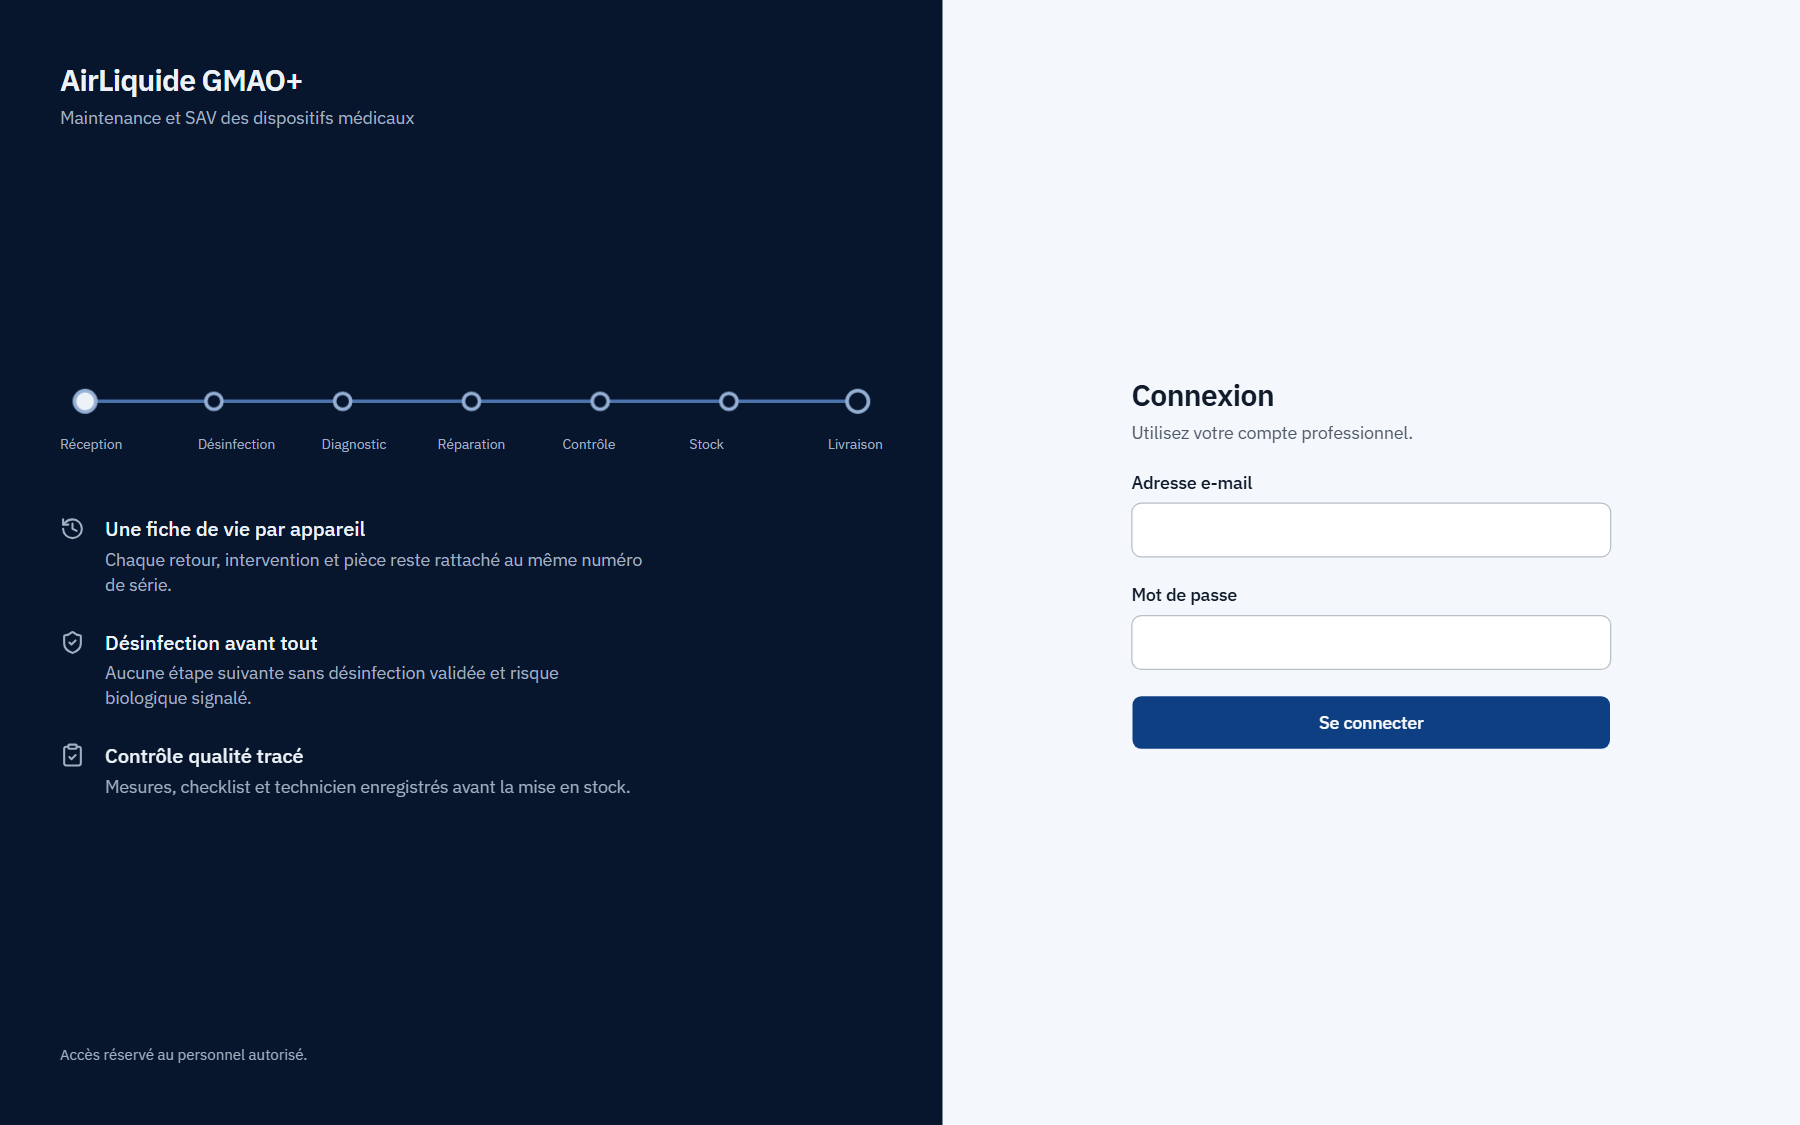
\includegraphics[width=15.0cm,height=17.5cm,keepaspectratio]{cap_connexion.png}
\caption{Écran de connexion}
\end{figure}

\begin{figure}[!htb]
\centering
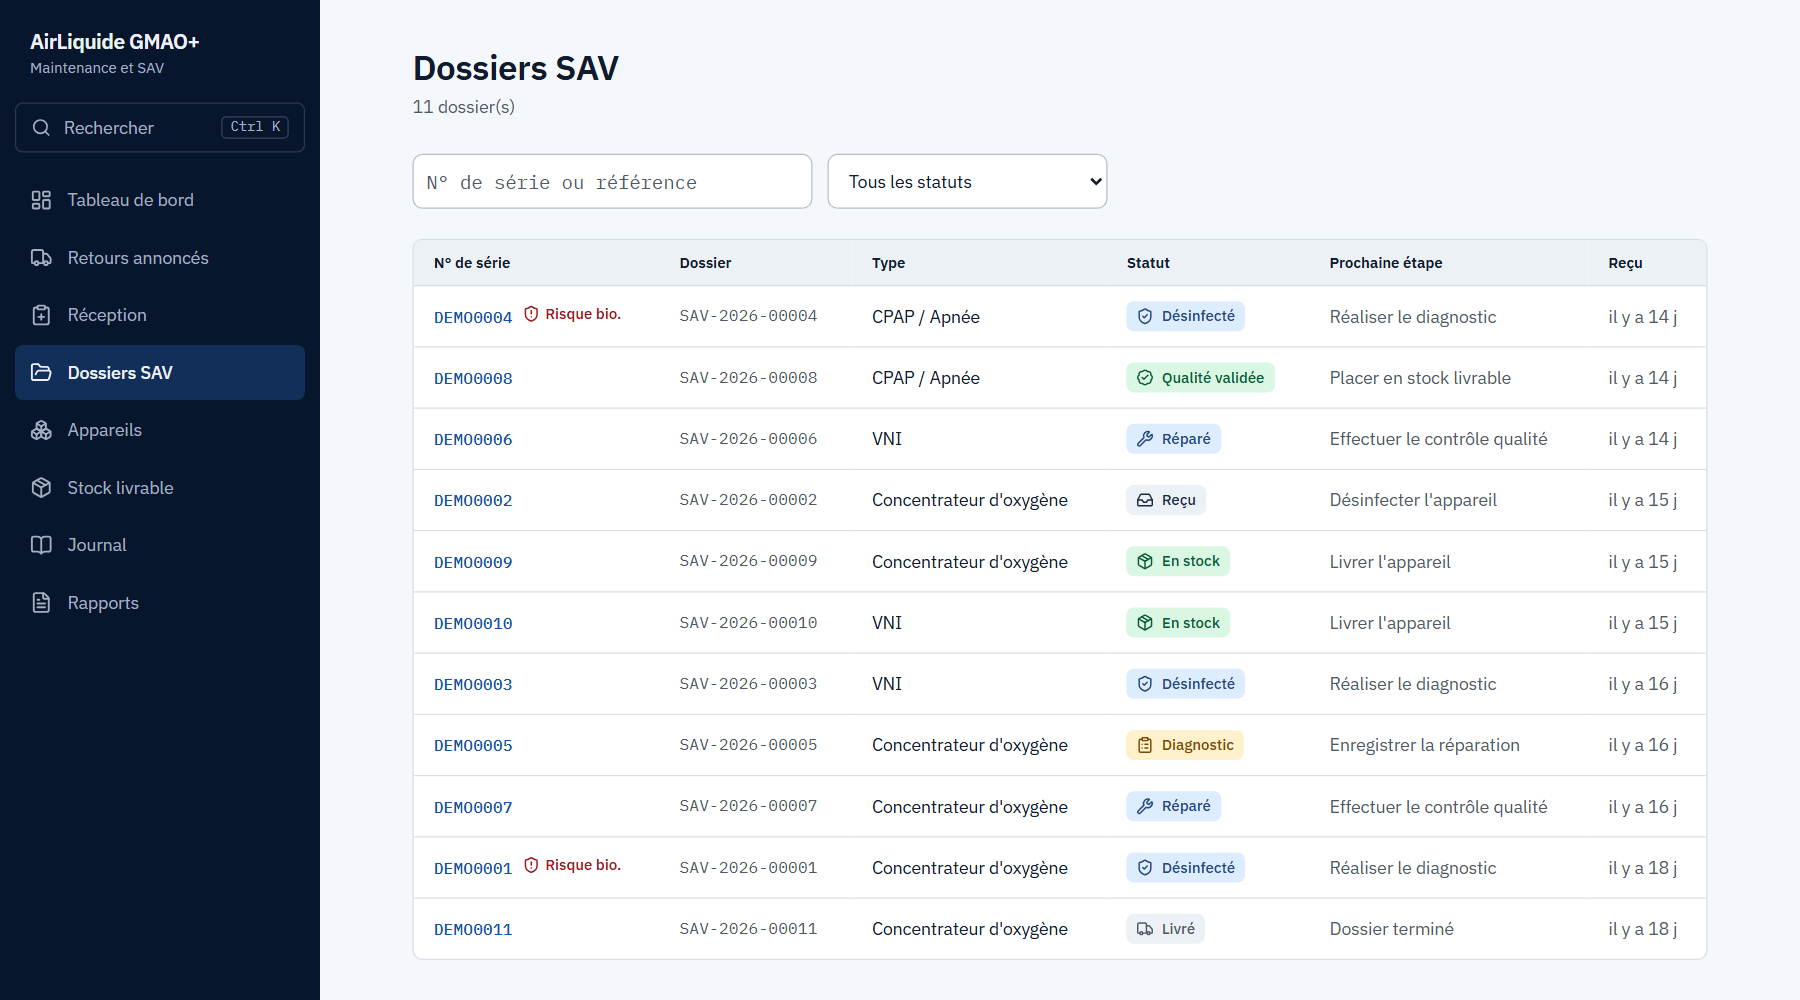
\includegraphics[width=15.0cm,height=17.5cm,keepaspectratio]{cap_dossiers.png}
\caption{Liste des dossiers SAV (données de démonstration)}
\end{figure}

\begin{figure}[!htb]
\centering
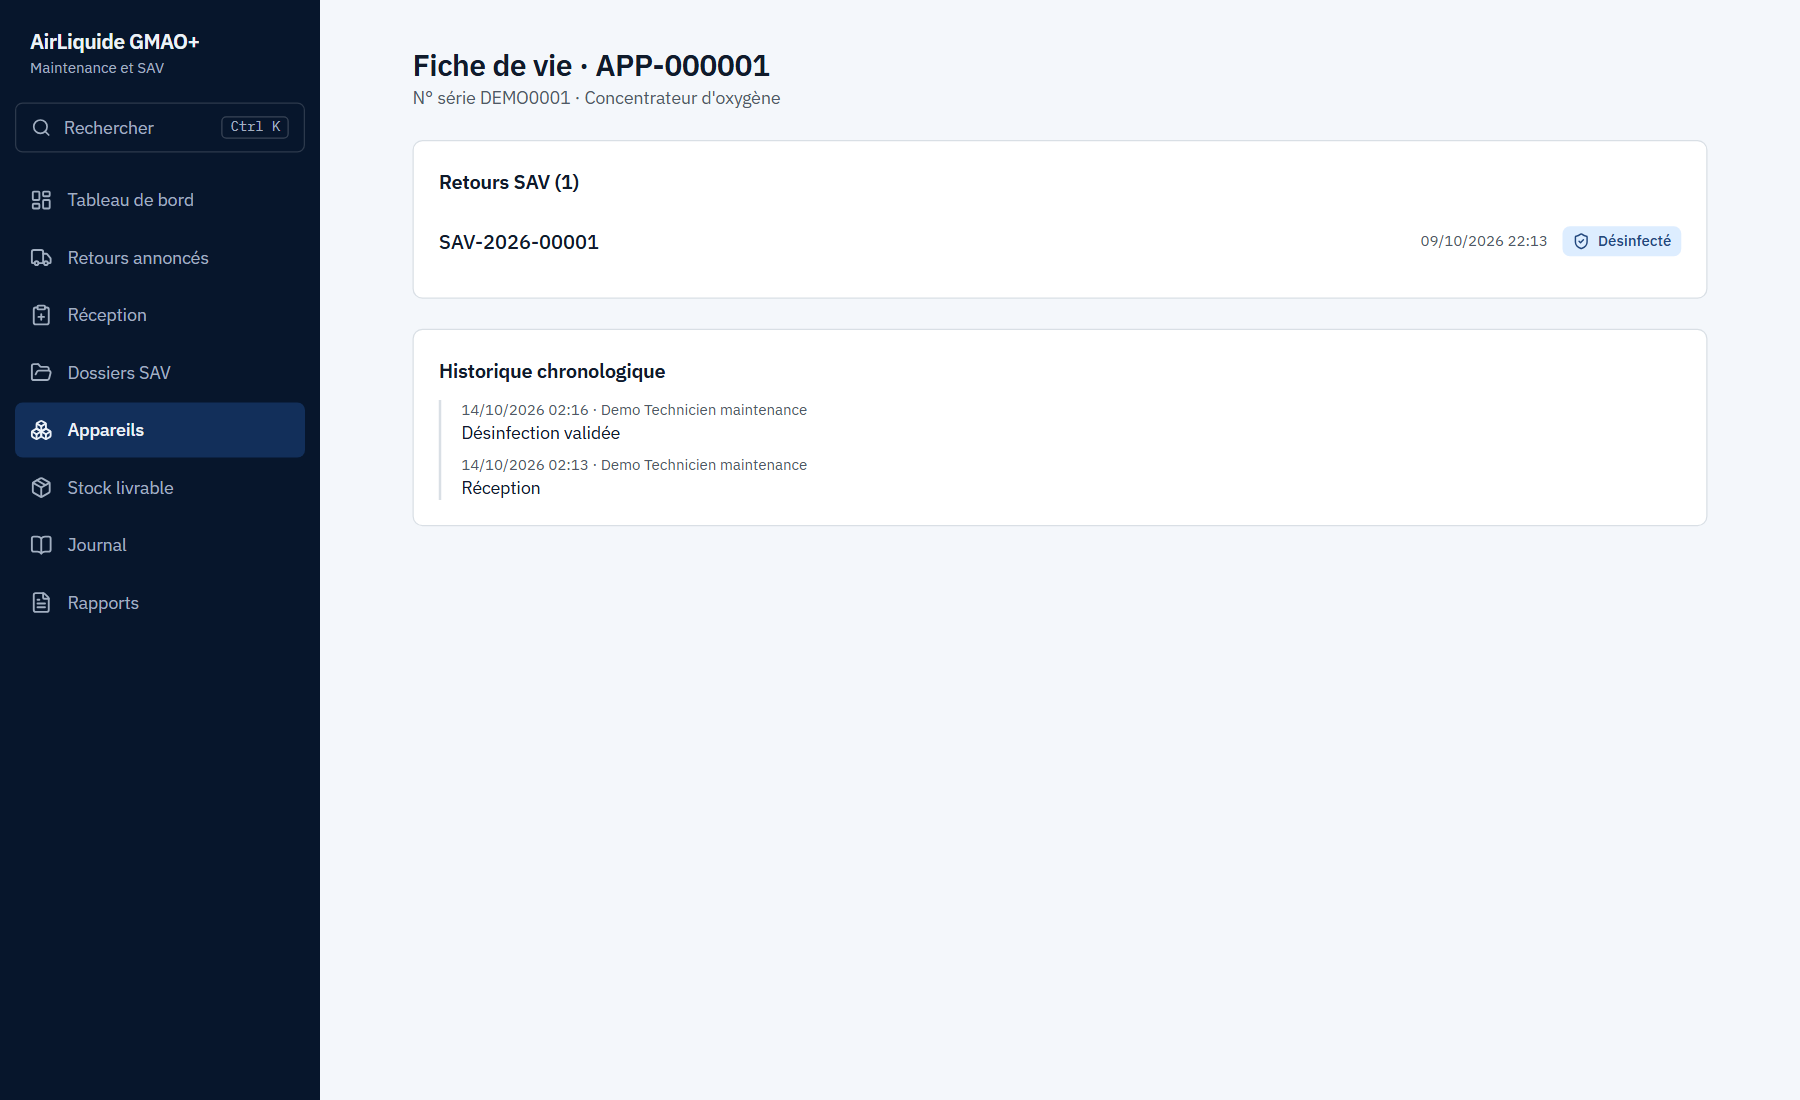
\includegraphics[width=15.0cm,height=17.5cm,keepaspectratio]{cap_fiche_vie.png}
\caption{Fiche de vie d'un appareil (données de démonstration)}
\end{figure}

\begin{figure}[!htb]
\centering
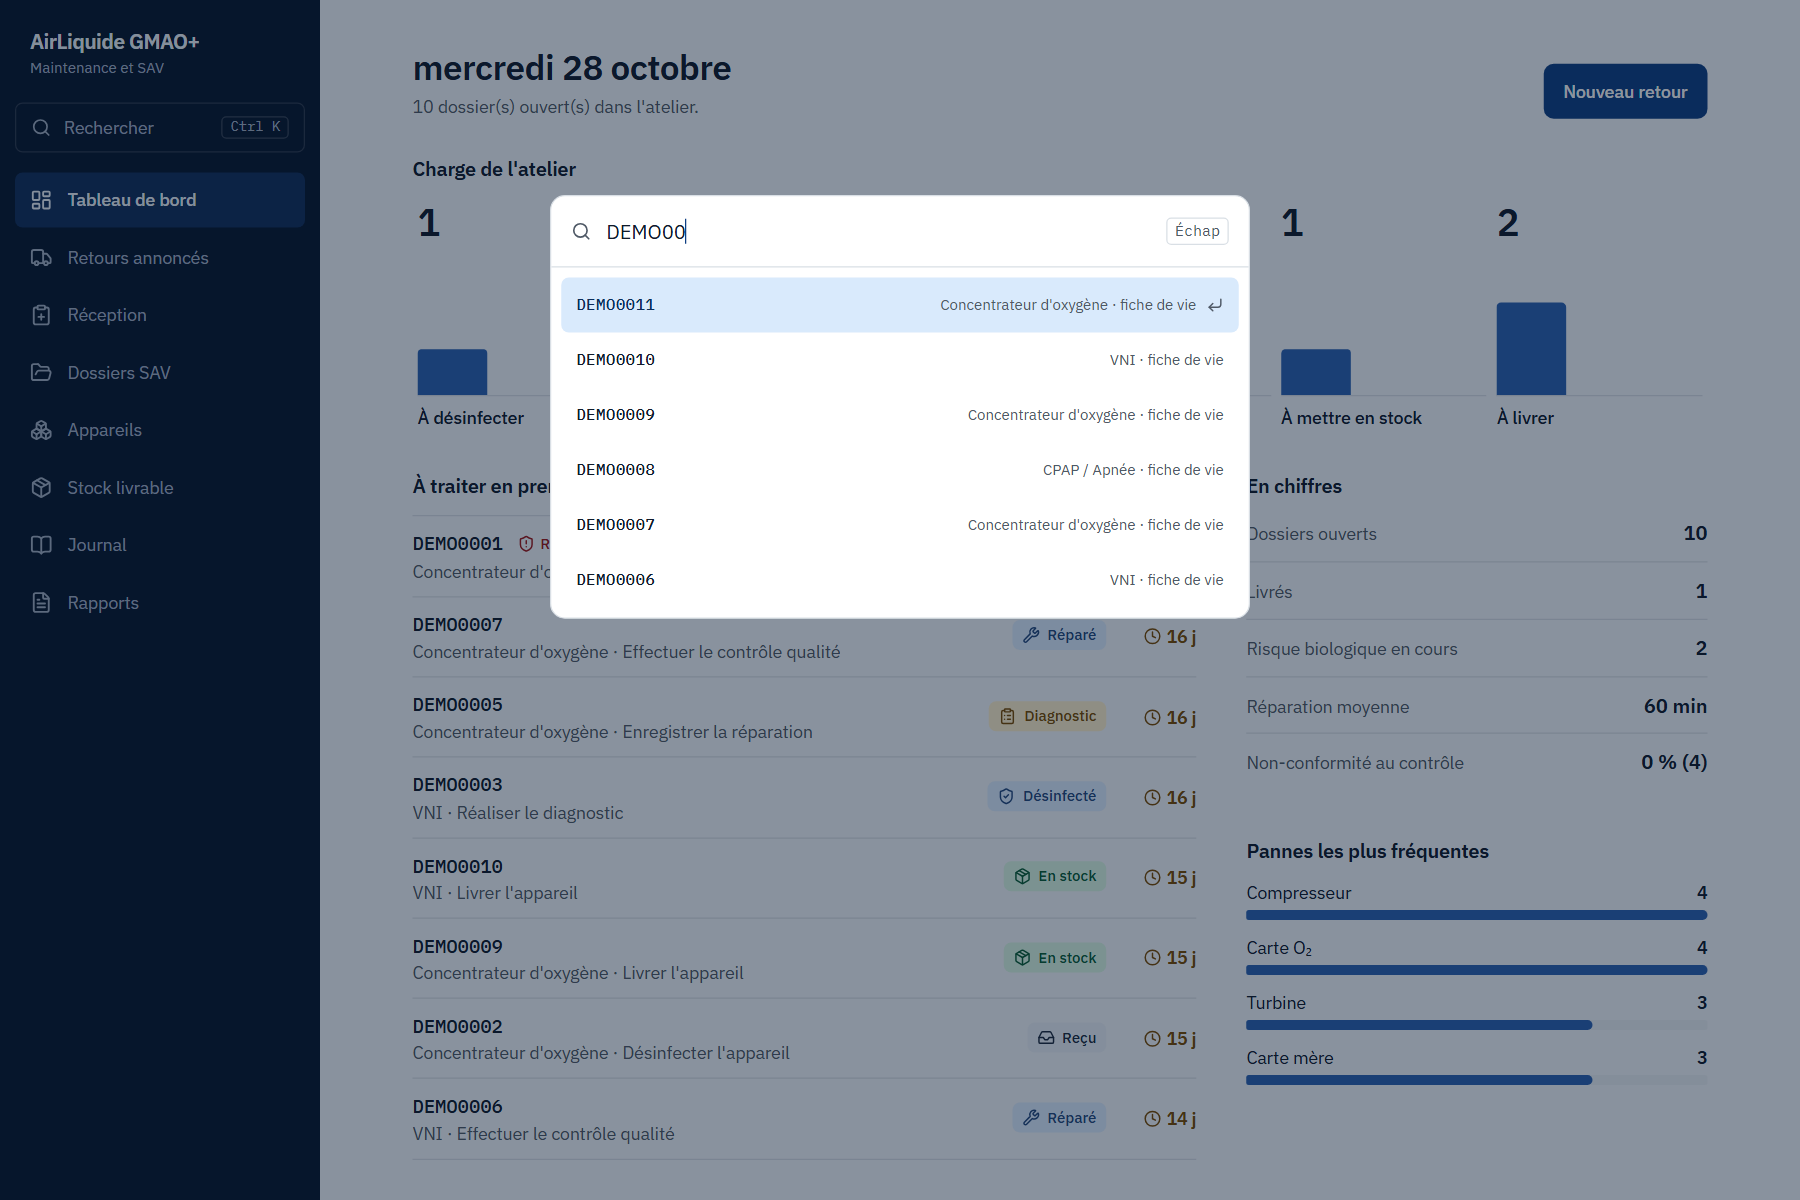
\includegraphics[width=15.0cm,height=17.5cm,keepaspectratio]{cap_palette.png}
\caption{Recherche rapide par numéro de série (Ctrl + K)}
\end{figure}

\begin{figure}[!htb]
\centering
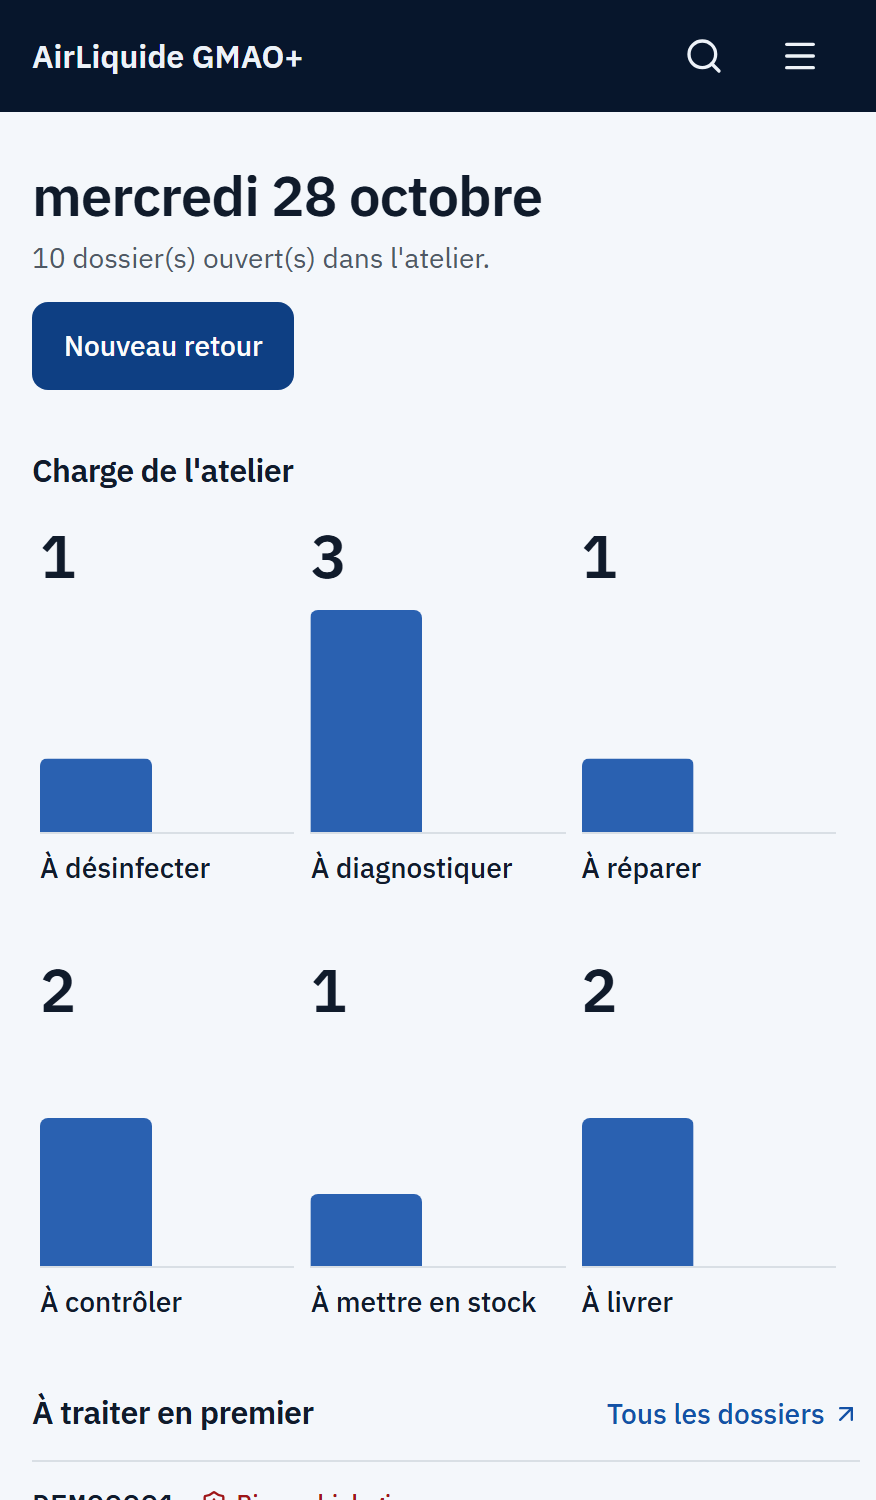
\includegraphics[width=7.5cm,height=17.0cm,keepaspectratio]{cap_mobile.png}
\caption{Tableau de bord sur téléphone}
\end{figure}

\section*{Annexe F : Exécution des tests automatisés}
\addcontentsline{toc}{section}{Annexe F : Exécution des tests automatisés}

Commande (depuis le dossier \texttt{backend/\allowbreak{}}) :

\texttt{python manage.\allowbreak{}py test}

Résultat observé le 28 octobre 2026, environnement SQLite : \texttt{Ran 49 tests} suivi de \texttt{OK}.

